\documentclass[conference]{IEEEtran}
\IEEEoverridecommandlockouts
% The preceding line is only needed to identify funding in the first footnote. If that is unneeded, please comment it out.
\usepackage{cite}
\usepackage{amsmath,amssymb,amsfonts}
\usepackage{algorithmic}
\usepackage{graphicx}
\usepackage{hyperref}
\usepackage{subcaption}
\usepackage{textcomp}
\usepackage{xcolor}
\def\BibTeX{{\rm B\kern-.05em{\sc i\kern-.025em b}\kern-.08em
    T\kern-.1667em\lower.7ex\hbox{E}\kern-.125emX}}

\hypersetup{
    colorlinks=true,
    linkcolor=blue,
    filecolor=magenta,
    urlcolor=cyan,
}

\begin{document}

\title{FaceNet Cluster Analysis}

\author{
\IEEEauthorblockN{Rodrigo Castiel}
\IEEEauthorblockA{\textit{Center for Informatics} \\
\textit{Federal University of Pernambuco} \\
Recife, Brazil \\
rcrs2@cin.ufpe.br}
}


\maketitle

\begin{abstract}
In the last decade, deep-learning based techniques brought us a remarkable breakthrough in face recognition.
Recently, Google Researchers proposed \textit{FaceNet}, a novel face recognition system that learns a mapping from face pictures to a feature-space where similarities are well described by simple euclidean distances \cite{b1}.
FaceNet may be combined with different clustering methods and classifiers; on famous face recognition databases, it currently achieves the best accuracy.
In this paper, we use FaceNet as a feature extractor to perform a face clustering analysis on three different databases: a small personal dataset, Labeled Faces in the Wild (LFW) and MUCT.
Our goal is to group pictures by identity.
We run k-means, agglomerative clustering, spectral clustering, DBSCAN and mean-shift with different parameters on all datasets.
Experiments show that both DBSCAN and mean-shift achieve the best adjusted rand scores without even requiring the number of clusters to be known in advance.

\end{abstract}

\begin{IEEEkeywords}
clustering, deep-learning, face recognition, facenet
\end{IEEEkeywords}

\section{Introduction}

Face recognition is a widely studied research field, whose large number of applications range from biometry to security.
While traditional techniques required a predetermined set of features which were manually chosen by humans, recent papers propose advanced systems capable of learning the most informative and even abstract attributes for classification \cite{b6}.
In 2015, Schroff et al. \cite{b1} developed a novel system called \textit{FaceNet}.
Unlike previous deep learning approaches, FaceNet introduces the harmonic triplet loss function, which is the key for learning the embedding with greater \textit{representional efficiency}.

According to the authors, FaceNet may be easily used for tasks like clustering and classification, since it is able to compute $128$-dimensional feature-vectors in an euclidean space where distances model the similarity between people.
The paper presents record holder classification results on famous databases such as Youtube Faces DB and Labeled Faces in the Wild (LFW), but
does not provide a detailed analysis of clustering methods.
A simple search on google scholar and other platforms show that only a few recent papers deal with the comparison of clustering methods on the state-of-art FaceNet system.
A.F. Bijl at \cite{b4} presents a good analysis, but it is focused only on the LFW and ISIS databases.

Therefore, in this project, we analyze the quality of clustering algorithms when FaceNet is used as feature extractor on multiple databases, each with arbitrary properties.
We perform a detailed study on three distinct databases, under two main perspecitives: the accuracy of cluster assignments and the semantics of assignment errors.
We compare k-means, agglomerative clustering, spectral clustering, DBSCAN and mean-shift \cite{b2, b3}.
Our experiments suggest that DBSCAN and mean-shift are the best options in most cases, since they achieve the highest accuracies without the need for knowing the number of clusters in advance.

\section{Clustering Analysis}

\subsection{Databases}

In this project, we chose three face databases with different properties to evaluate the quality of the clustering methods.
The first database, \textit{personal\_faces}, is a small dataset containing arbitrary pictures of our teammates and classmates under random lighting and environmental conditions.
The second database is \textit{Labeled Faces in the Wild} (LFW) \cite{b5}, a large database of famous people under random circumstances.
The third database is \textit{MUCT} \cite{b7}, a reasonably large dataset of people under multiple predetermined lighting and camera angles.
Both \textit{personal\_faces} and LFW contain an uneven number of face pictures per person, while MUCT has the same picture styles for every person.
We picked \textit{personal\_faces} to perform a semantics analysis of the error pictures in a simple and clear way.

Given the raw database, we use OpenCV's cascade classifier to detect faces in the pictures \cite{b8}.
It does not always find valid faces in an image, which makes the number of extracted faces to be slightly lower than the actual dataset size.
\textit{personal\_faces} contains $N = 59$ face pictures distributed over $K = 18$ clusters (people).
MUCT contains $N = 3710$ faces distributed over $K = 276$ clusters.
LFW originally contains $N = 13233$ faces distributed over $K = 5749$ people, but we filter out clusters with less than three pictures.
Therefore, the processed LFW database contains $N = 7400$ faces from $K = 901$ people.

Figure \ref{tsneview} (a) is a visualization of the \textit{personal\_faces} dataset in feature-space.
Notice that clusters are located in disjoint regions with clear boundaries.
Figure \ref{tsneview} (b) shows the clusters in LFW.
Due to its large volume, its several different ethnical groups and picture angles, it presents multiple overlaps between clusters.
The size and the scattering of its clusters are uneven.
Figure \ref{tsneview} (c) depicts MUCT.
There is much less overlapping than in LFW; in general, clusters are dense and clearly separable.

\begin{figure}
  \begin{subfigure}[b]{0.5\textwidth}
    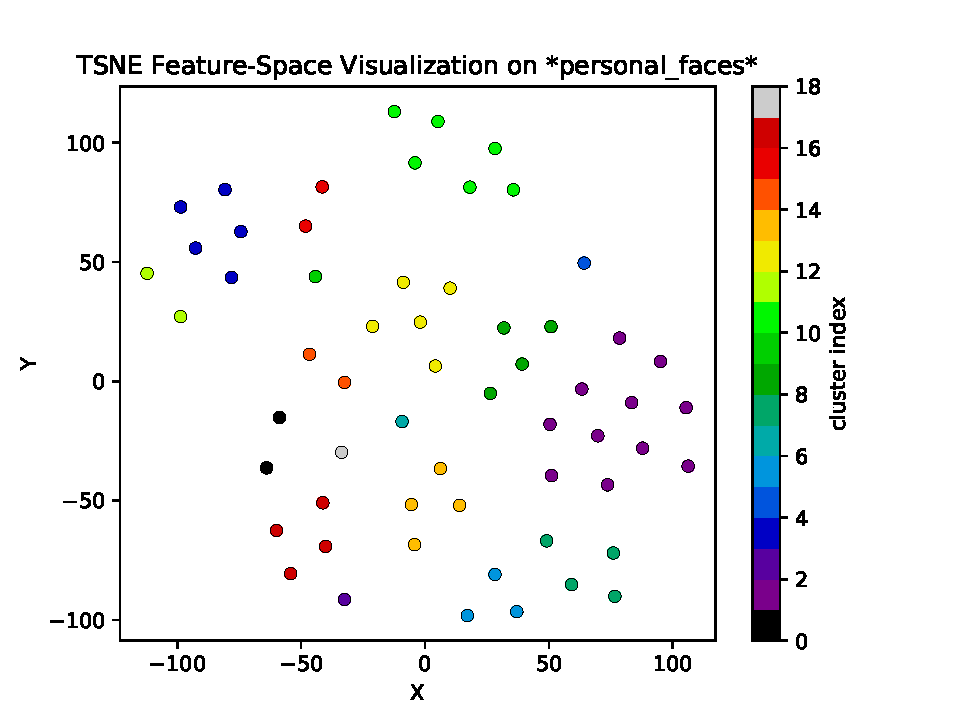
\includegraphics[width=\linewidth]{tsne_view_personal_faces}
    \caption{}
  \end{subfigure}
  \begin{subfigure}[b]{0.5\textwidth}
    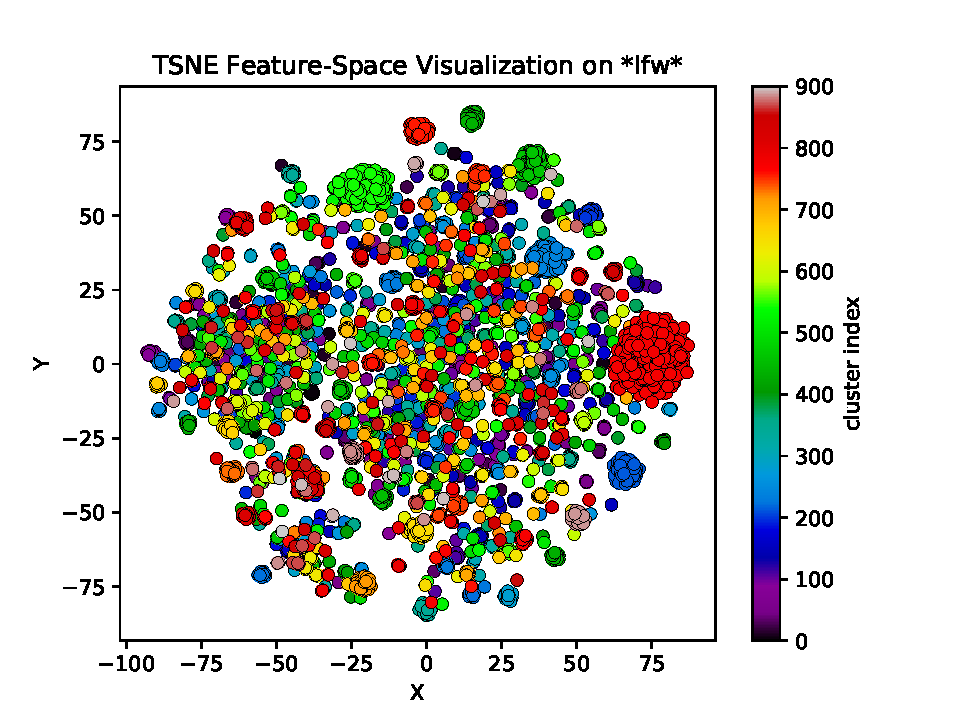
\includegraphics[width=\linewidth]{tsne_view_lfw}
    \caption{}
  \end{subfigure}
  \begin{subfigure}[b]{0.5\textwidth}
    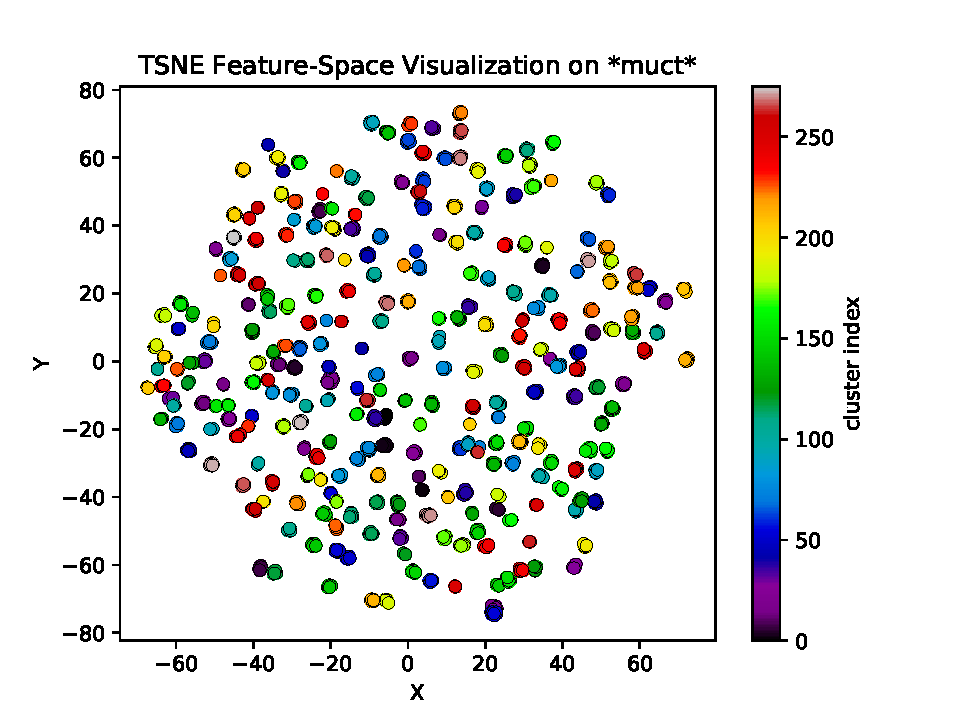
\includegraphics[width=\linewidth]{tsne_view_muct}
    \caption{}
  \end{subfigure}
  \caption{TSNE visualization of multiple databases in a reduced 2D feature-space. Cluster indices are assigned to random colors. (a) personal\_faces. (b) LFW. (c) MUCT.}
  \label{tsneview}
\end{figure}

\subsection{Experiments}

\begin{figure}
  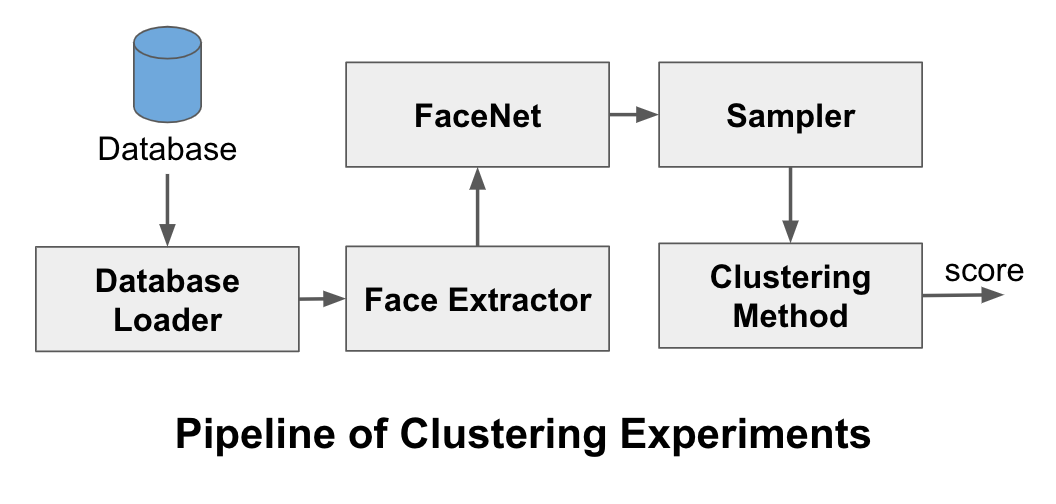
\includegraphics[width=\linewidth]{pipeline.png}
  \caption{Test subset creation pipeline. In the first step, raw images are loaded from the database. Then, OpenCV's cascade classifier is applied on the images to extract faces and resize them to $160\times160$. Afterwards, we evaluate FaceNet on each face picture to get the embeddings (feature-vectors). In each run, we sample a random subset of embeddings and feed it to clustering methods.}
  \label{pipeline}
\end{figure}

In order to properly assess the quality of the clustering techniques, we evaluate the \textit{adjusted rand index} (or simply $ARI$ \cite{b9}) of each method on a series of random subsets sampled from the entire input databases.
Each clustering method, with its given parameter values, is executed $n_{eval} = 30$ times on a randomly sampled subset whose size is approximately $80\%$ of the total database size.
At the end, we compute the average $ARI$ score of each set of runs.
Figure \ref{pipeline} depicts the stages of our clustering experiments.
We use a precomputed \textit{FaceNet} model trained on the Microsoft's MS-Celeb-1M database.
This model was implemented by \textit{nyoki-mtl}, and is available on his github page \cite{b10}.
It takes a $160 \times 160$ picture as input, and outputs a $128$-dimensional feature vector.

Recall that k-means, agglomerative clustering and spectral clustering need a hyper-parameter $K$, that is, the number of clusters to be found.
If $K$ is less than the actual number of people, these methods will tend to group similar people into the same clusters.
For example, pictures of people who share the same ethnical group, or who grow beard.
Though we could exhaustively tweak $K$ until we find the best $ARI$ score, we will not have a reference in practice, since no ground-truth labels are provided.
Therefore, for comparison purposes, we assume that $K$ is known.
Thus, this will give us a good upperbound for their scores.

On the other hand, we run mean-shift and DBSCAN with different hyper-parameter values.
As described in the following section, experiments suggest that both of them are roughly invariant to the real number of clusters.
In other words, their best hyper-parameters are about the same for any database.

\subsection{Results}

\textbf{Score Analysis}. As previously mentioned, the average $ARI$ and the standard deviation are computed for each series of runs, depicted as entries of Table \ref{scores_table}.
On the \textit{personal\_faces} database, DBSCAN with $eps = 0.8$ achieves $ARI_{DBSCAN} = 0.903226$, outperforming all the other methods.
Mean-shift with $bw = 0.8$ achieves $ARI_{ms} = 0.898702$, a similar result.
Spectral clustering produces the worst score: $ARI_{spectral} = 0.697063$.
On LFW, mean-shift for $bw = 0.7$ achieves $ARI_{ms} = 0.980598$, followed by DBSCAN for $eps = 0.7$ with $ARI_{DBSCAN} = 0.956498$.
K-means, agglomerative clustering and spectral clustering produce poor results, with $ARI < 0.50$.
On MUCT, all methods yield roughly similar results, but agglomerative clustering achieves a slightly better score, with $ARI_{agg} = 0.987609$.

As showed in Table \ref{scores_table}, even when the number of clusters $K$ is known a priori, k-means, agglomerative and spectral clustering generally have lower scores.
However, DBSCAN and mean-shift are able to achieve good results without the need for tuning their hyper-parameters.
For example, mean-shift with $bw =0.7$ outpeforms the $K$-based methods on \textit{personal\_faces} and LFW, and achieves similar scores on MUCT.
Since MUCT is a database containing only a predetermined set of lighting and camera configurations, it is expected that all methods would perform well on it.
Yet, in practice, real picture datasets tend to follow the characteristics of \textit{personal\_faces} and LFW.
That is, they contain highly scattered clusters with unbalanced number of pictures per person.
Also, the number of people is not known in advance.
Therefore, DBSCAN and mean-shift may be the best options for organizing a list of random face pictures into groups of people.

\begin{table*}[t]
  \centering
  \begin{tabular}{ | l*{4}{c} | }
    \hline
                         & \vline &                          & Average $ARI$ ($2*std$) &     \\
    \hline
    METHOD (parameter)   & \vline & \textit{personal\_faces} & LFW                    & MUCT \\
    \hline
    k-means (opt)        & \vline & 0.815486 (+/- 0.230988) & 0.393992 (+/- 0.047119) & 0.966178 (+/- 0.009708) \\
    agglomerative (opt)  & \vline & 0.812108 (+/- 0.212971) & 0.440203 (+/- 0.030589) & 0.987609 (+/- 0.006514) \\
    spectral (opt)       & \vline & 0.697063 (+/- 0.236279) & 0.227804 (+/- 0.053009) & 0.974029 (+/- 0.012965) \\
    \hline
    DBSCAN $eps = 0.1$   & \vline & 0.344276 (+/- 0.136712) & 0.031102 (+/- 0.003716) & 0.134093 (+/- 0.008032) \\
    DBSCAN $eps = 0.2$   & \vline & 0.314153 (+/- 0.158736) & 0.031848 (+/- 0.003995) & 0.166055 (+/- 0.010299) \\
    DBSCAN $eps = 0.3$   & \vline & 0.283740 (+/- 0.130011) & 0.032313 (+/- 0.003964) & 0.476711 (+/- 0.036143) \\
    DBSCAN $eps = 0.4$   & \vline & 0.333242 (+/- 0.150010) & 0.196961 (+/- 0.056513) & 0.802872 (+/- 0.020068) \\
    DBSCAN $eps = 0.5$   & \vline & 0.432967 (+/- 0.174418) & 0.724950 (+/- 0.032456) & 0.940610 (+/- 0.010532) \\
    DBSCAN $eps = 0.6$   & \vline & 0.614341 (+/- 0.247413) & 0.908426 (+/- 0.013233) & 0.979826 (+/- 0.007118) \\
    DBSCAN $eps = 0.7$   & \vline & 0.803644 (+/- 0.177654) & 0.956498 (+/- 0.011196) & 0.980598 (+/- 0.008401) \\
    DBSCAN $eps = 0.8$   & \vline & 0.903226 (+/- 0.109752) & 0.853182 (+/- 0.096127) & 0.651178 (+/- 0.142826) \\
    DBSCAN $eps = 0.9$   & \vline & 0.783702 (+/- 0.194788) & 0.129282 (+/- 0.082319) & 0.071823 (+/- 0.019167) \\
    DBSCAN $eps = 1.0$   & \vline & 0.597496 (+/- 0.269718) & 0.002835 (+/- 0.000719) & 0.002495 (+/- 0.000438) \\
    DBSCAN $eps = 1.1$   & \vline & 0.267060 (+/- 0.256646) & 0.000009 (+/- 0.000019) & 0.000003 (+/- 0.000022) \\
    DBSCAN $eps = 1.2$   & \vline & 0.099561 (+/- 0.130185) & 0.000000 (+/- 0.000000) & 0.000000 (+/- 0.000000) \\
    \hline
    mean-shift $bw =0.1$ & \vline & 0.317914 (+/- 0.140322) & 0.030939 (+/- 0.003717) & 0.134485 (+/- 0.006195) \\
    mean-shift $bw =0.2$ & \vline & 0.315753 (+/- 0.159228) & 0.031276 (+/- 0.002873) & 0.168938 (+/- 0.008185) \\
    mean-shift $bw =0.3$ & \vline & 0.324247 (+/- 0.154227) & 0.033189 (+/- 0.004090) & 0.502991 (+/- 0.027087) \\
    mean-shift $bw =0.4$ & \vline & 0.321497 (+/- 0.201095) & 0.254383 (+/- 0.048598) & 0.829826 (+/- 0.020178) \\
    mean-shift $bw =0.5$ & \vline & 0.437489 (+/- 0.223821) & 0.760404 (+/- 0.028746) & 0.952445 (+/- 0.011531) \\
    mean-shift $bw =0.6$ & \vline & 0.710785 (+/- 0.240384) & 0.922974 (+/- 0.013579) & 0.982613 (+/- 0.006856) \\
    mean-shift $bw =0.7$ & \vline & 0.840041 (+/- 0.186023) & 0.960519 (+/- 0.011309) & 0.981194 (+/- 0.009435) \\
    mean-shift $bw =0.8$ & \vline & 0.898702 (+/- 0.103473) & 0.915924 (+/- 0.022172) & 0.442032 (+/- 0.079450) \\
    mean-shift $bw =0.9$ & \vline & 0.684107 (+/- 0.285094) & 0.553595 (+/- 0.115690) & 0.072555 (+/- 0.012895) \\
    mean-shift $bw =1.0$ & \vline & 0.175552 (+/- 0.215836) & 0.003532 (+/- 0.001298) & 0.001111 (+/- 0.000390) \\
    mean-shift $bw =1.1$ & \vline & 0.003220 (+/- 0.019918) & 0.000000 (+/- 0.000000) & 0.000000 (+/- 0.000000) \\
    mean-shift $bw =1.2$ & \vline & 0.000000 (+/- 0.000000) & 0.000000 (+/- 0.000000) & 0.000000 (+/- 0.000000) \\
    \hline
  \end{tabular}
  \caption{Average $ARI$ score of all methods on different databases (together with their standard deviations). Each row represents a clustering technique with a specific parameter value, while each column is a database. In DBSCAN rows, $eps$ means the maximum possible distance between points in the same cluster. In mean-shift rows, $bw$ stands for bandwidth. }
  \label{scores_table}
\end{table*}

\textbf{Mean-shift and DBSCAN hyper-parameter analysis}. To understand the impact of $bw$ (bandwidth) and $eps$ (minimum distance between points in the same cluster) on mean-shift and DBSCAN, respectively, we plot the scores \textit{vs} the parameter values on different datasets (Figure \ref{parameter_plot}).
An interesting pattern arising from the plots is that the more spread-out the clusters are, the larger the optimal $bw$ and $eps$ will be.
That is, the peaks show up at higher values of bandwidth and $eps$.
Nonetheless, these parameters are not so sensitive (peaks are wide).
As mentioned above, real world pictures tend to generate scattered, sometimes overlapped clusters.
Therefore, higher distance parameters such as $bw, eps \approx 0.7$ are usually preferred.

In both cases if the parameters are too small, then the algorithms will try to split large clusters into smaller subgroups.
If the parameters are large enough, the algorithms will merge weakly related clusters.
For this reason, if the parameters are not well chosen, these algorithms will produce extremely inaccurate results.

\begin{figure}
  \begin{subfigure}[b]{0.45\textwidth}
    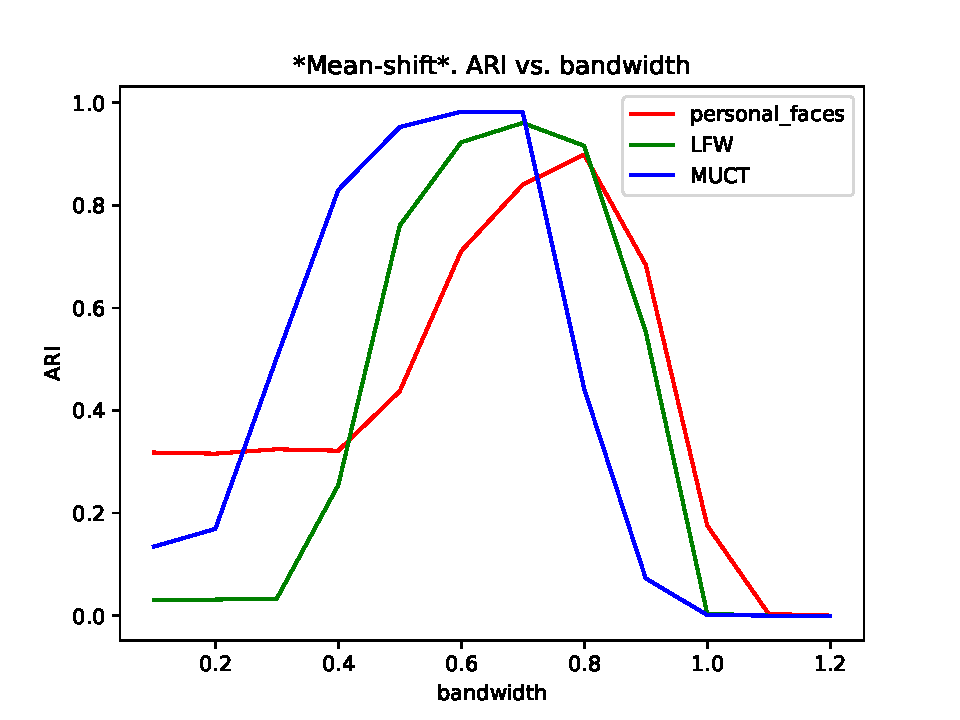
\includegraphics[width=\linewidth]{meanshift-plot}
    \caption{}
  \end{subfigure}
  \begin{subfigure}[b]{0.45\textwidth}
    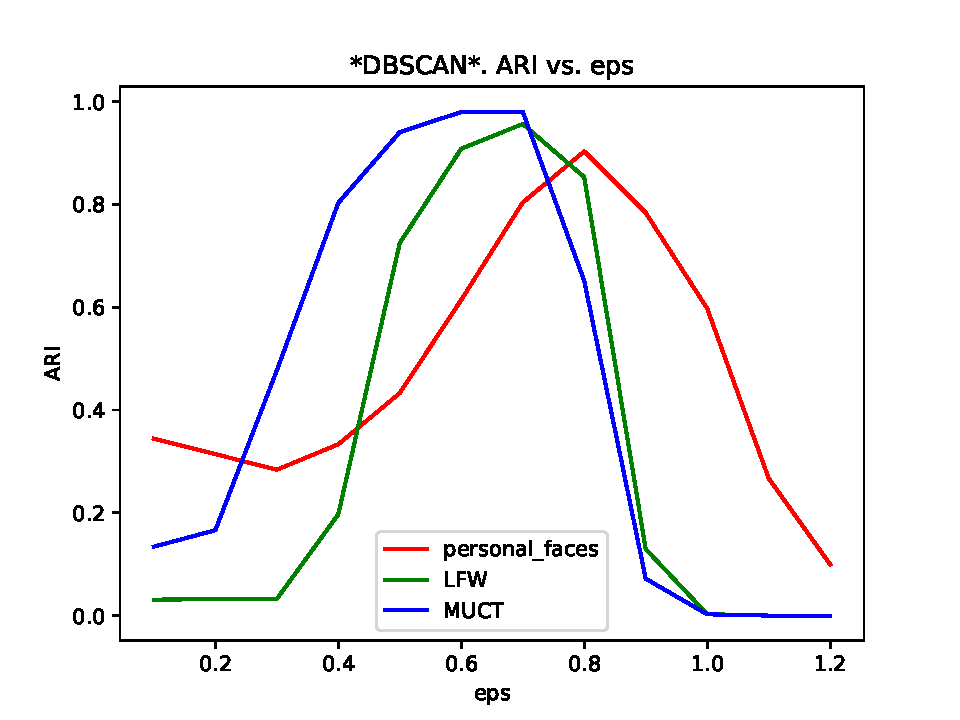
\includegraphics[width=\linewidth]{dbscan-plot}
    \caption{}
  \end{subfigure}
  \caption{Plots of \textit{ARI} scores \textit{vs.} hyper-parameters. \textit{personal\_faces}, LFW and MUCT are displayed in red, green and blue, respectively. The vertical axis indicates the score value, and the horizontal axis indicates the method-specific parameter values. (a) Mean-shift. (b) DBSCAN. }
  \label{parameter_plot}
\end{figure}


\textbf{Semantics Analysis}. To help visualize how errors are manifested over different techniques, we created a tool that organizes databases by grouping photos that share the same person.
We tested it on \textit{personal\_faces} and analyzed results manually and qualitatively.
In all cases, we notice that wrong picture assignments are usually correlated with similar face traits such as shape (of head, nose and mouth), beard color, the presence of glasses and the ethnicity.
For more details, see Figures \ref{wrong_similar} and \ref{wrong_ethnical}.
In this sense, FaceNet does a great job estimating informative and high-quality embeddings (feature vectors).

Regarding DBSCAN and mean-shift, the main downside is that they may overestimate the number of clusters depending on the parameter values.
Although their scores are high on small datasets, they can end up splitting up real clusters into smaller subgroups.
This also happens sometimes with $K$-based algorithms.
An underlying problem which no technique avoided is assigning the same person with and without sunglasses to different clusters (Figure \ref{wrong_split}).

\begin{figure}
  \centering
  \begin{subfigure}[b]{0.2\textwidth}
    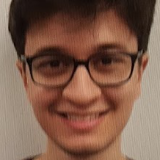
\includegraphics[width=\linewidth]{wrong_similar_a}
  \end{subfigure}
  \begin{subfigure}[b]{0.2\textwidth}
    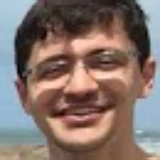
\includegraphics[width=\linewidth]{wrong_similar_b}
  \end{subfigure}
  \caption{Different people assigned to the same k-means cluster. Notice the face similarity: the nose and mouth shape are close; also both use glasses.}
  \label{wrong_similar}
\end{figure}

\begin{figure}
  \centering
  \begin{subfigure}[b]{0.2\textwidth}
    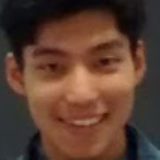
\includegraphics[width=\linewidth]{wrong_ethnical_a}
  \end{subfigure}
  \begin{subfigure}[b]{0.2\textwidth}
    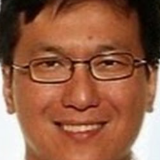
\includegraphics[width=\linewidth]{wrong_ethnical_b}
  \end{subfigure}
  \caption{Different people assigned to the same group by agglomerative clustering. Both people share the same ethnical group, though they are clearly distinguishable by humans.}
  \label{wrong_ethnical}
\end{figure}

\begin{figure}
  \centering
  \begin{subfigure}[b]{0.2\textwidth}
    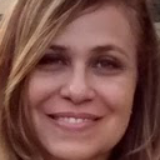
\includegraphics[width=\linewidth]{wrong_split_a}
  \end{subfigure}
  \begin{subfigure}[b]{0.2\textwidth}
    
\includegraphics[width=\linewidth]{wrong_split_b}
  \end{subfigure}
  \caption{Same person assigned to different clusters because of sunglasses. As humans, we clearly see that the hairstyle, the smile and the nose shapes are all preserved in both pictures. This mistake was made by all methods, which shows that the corresponding FaceNet embeddings are intrinsically distant.}
  \label{wrong_split}
\end{figure}

\section{Conclusion}

When $K$ is not known a priori, DBSCAN and mean-shift are the best scoring options for face clustering of large databases.
Their hyper-parameters are not sensitive to different input datasets.
However, if $K$ is known, agglomerative cluster is a good option since it does not overestimate the number of clusters.
Similarly DBSCAN, it is also able to find arbitrarily shaped clusters.

Our experiments suggest that, regardless of method, the FaceNet model trained on MS-Celeb-1M is sensitive to sunglasses.
Moreover, classification ends up being more accurate than clustering, because it handles overlapping better.
For example, a simple k-NN classifier would be able to correctly predict faces of similar people by votation, whereas clustering methods would not clearly know whether data samples belong to the same person or not.
As future work, we plan to study the impact of face expression and accessories on the embeddings computed by FaceNet trained on different databases.
We also want to analyze how the $ARI$ scores and metrics such as recall and precision change when the number of clusters increase.

\begin{thebibliography}{00}

\bibitem{b1} F. Schroff, D. Kalenichenko, and J. Philbin. Facenet: A unified embedding for face recognition and clustering. arXivpreprint arXiv:1503.03832, 2015.

\bibitem{b2} A.K. Jain, Data clustering: 50 years beyond k-means, Pattern Recognition. Lett. 31
(2010) 651–666

\bibitem{b3} Cheng, Yizong (August 1995). "Mean Shift, Mode Seeking, and Clustering". IEEE Transactions on Pattern Analysis and Machine Intelligence. IEEE. 17 (8): 790–799. doi:10.1109/34.400568

\bibitem{b4} A.F. Bijl, A. (2018). A comparison of clustering algorithms for face clustering. [online] Fse.studenttheses.ub.rug.nl. Available at: http://fse.studenttheses.ub.rug.nl/18064/1/Report\_research\_internship.pdf [Accessed 18 Nov. 2018].

\bibitem{b5} Gary B. Huang, Manu Ramesh, Tamara Berg, and Erik Learned-Miller.
Labeled Faces in the Wild: A Database for Studying Face Recognition in Unconstrained Environments.
University of Massachusetts, Amherst, Technical Report 07-49, October, 2007.

\bibitem{b6} Wang, M. and Deng, W. (2018). Deep Face Recognition: A Survey. [online] Arxiv.org. Available at: https://arxiv.org/abs/1804.06655 [Accessed 18 Nov. 2018].

\bibitem{b7} Milborrow, Stephen \& Morkel, John \& Nicolls, Fred. (2018). The MUCT Landmarked Face Database.

\bibitem{b8} Docs.opencv.org. (2018). Cascade Classifier — OpenCV 2.4.13.7 documentation. [online] Available at: https://docs.opencv.org/2.4/doc/tutorials/objdetect/cascade\_classifier/cascade\_classifier.html [Accessed 18 Nov. 2018].

\bibitem{b9} W. M. Rand (1971). "Objective criteria for the evaluation of clustering methods". Journal of the American Statistical Association. American Statistical Association. 66 (336): 846–850. doi:10.2307/2284239. JSTOR 2284239

\bibitem{b10} GitHub. (2018). nyoki-mtl/keras-facenet. [online] Available at: https://github.com/nyoki-mtl/keras-facenet [Accessed 18 Nov. 2018].

\end{thebibliography}

\end{document}
